\documentclass[sigplan,review,nonacm,10pt]{acmart}

\usepackage{minted}
\usepackage{makecell}
\usepackage{booktabs}
\usepackage{microtype}
\graphicspath{ {./figs/} }
\newcommand\aste{%
$^{(\ast)}$
}
\usepackage[subtle]{savetrees}

% https://tex.stackexchange.com/questions/655620/how-to-make-acmart-stop-complaining-about-missing-country-in-affiliation
\makeatletter
\def\@ACM@checkaffil{% Only warnings
    \if@ACM@instpresent\else
    \ClassWarningNoLine{\@classname}{No institution present for an affiliation}%
    \fi
    \if@ACM@citypresent\else
    \ClassWarningNoLine{\@classname}{No city present for an affiliation}%
    \fi
    \if@ACM@countrypresent\else
        \ClassWarningNoLine{\@classname}{No country present for an affiliation}%
    \fi
}
\makeatother

%%
%% \BibTeX command to typeset BibTeX logo in the docs
\AtBeginDocument{%
  \providecommand\BibTeX{{%
    Bib\TeX}}}

%% Rights management information.  This information is sent to you
%% when you complete the rights form.  These commands have SAMPLE
%% values in them; it is your responsibility as an author to replace
%% the commands and values with those provided to you when you
%% complete the rights form.
\setcopyright{acmcopyright}
\copyrightyear{2023}
\acmYear{2023}
%\acmDOI{XXXXXXX.XXXXXXX}

%% These commands are for a PROCEEDINGS abstract or paper.
\acmConference[CS294]{CS294}{Fall 2023}{Berkeley, CA}
%%
%%  Uncomment \acmBooktitle if the title of the proceedings is different
%%  from ``Proceedings of ...''!
%%
%%\acmBooktitle{Woodstock '18: ACM Symposium on Neural Gaze Detection,
%%  June 03--05, 2018, Woodstock, NY}
%\acmPrice{15.00}
%\acmISBN{978-1-4503-XXXX-X/18/06}


%%
%% Submission ID.
%% Use this when submitting an article to a sponsored event. You'll
%% receive a unique submission ID from the organizers
%% of the event, and this ID should be used as the parameter to this command.
%%\acmSubmissionID{123-A56-BU3}

%%
%% For managing citations, it is recommended to use bibliography
%% files in BibTeX format.
%%
%% You can then either use BibTeX with the ACM-Reference-Format style,
%% or BibLaTeX with the acmnumeric or acmauthoryear sytles, that include
%% support for advanced citation of software artefact from the
%% biblatex-software package, also separately available on CTAN.
%%
%% Look at the sample-*-biblatex.tex files for templates showcasing
%% the biblatex styles.
%%

%%
%% The majority of ACM publications use numbered citations and
%% references.  The command \citestyle{authoryear} switches to the
%% "author year" style.
%%
%% If you are preparing content for an event
%% sponsored by ACM SIGGRAPH, you must use the "author year" style of
%% citations and references.
%% Uncommenting
%% the next command will enable that style.
%%\citestyle{acmauthoryear}
\settopmatter{printacmref=false}

%%
%% end of the preamble, start of the body of the document source.
\begin{document}

%%
%% The "title" command has an optional parameter,
%% allowing the author to define a "short title" to be used in page headers.
% \title{TidalSim: Mixing Functional Simulation, $\mu$Arch Models, and RTL Simulation for Rapid Microarchitectural Iteration and Evaluation}
\title{TidalSim: Multi-Level Simulation for Rapid Microarchitectural Iteration and Evaluation}

%%
%% The "author" command and its associated commands are used to define
%% the authors and their affiliations.
%% Of note is the shared affiliation of the first two authors, and the
%% "authornote" and "authornotemark" commands
%% used to denote shared contribution to the research.

%Young-Jin Park, Rohit Agarwal, Oliver Yu, Lixiang (Andy) Yin, and Bryan Ngo have worked on the eDSLs presented in this paper.
\author{\href{https://orcid.org/0000-0001-6934-6577}{Vighnesh Iyer}, Raghav Gupta, Dhruv Vaish, \href{https://orcid.org/0000-0003-2324-1715}{Borivoje Nikolić}}
\email{{vighnesh.iyer,rgupta,dvaish,bora}@berkeley.edu}
\affiliation{%
  \institution{UC Berkeley}
}

% \author{Borivoje Nikolić}
% \email{bora@eecs.berkeley.edu}
% \orcid{0000-0003-2324-1715}
% \affiliation{%
%   \institution{UC Berkeley}
% }


%%
%% By default, the full list of authors will be used in the page
%% headers. Often, this list is too long, and will overlap
%% other information printed in the page headers. This command allows
%% the author to define a more concise list
%% of authors' names for this purpose.
\renewcommand{\shortauthors}{Iyer, Vighnesh et al.}

\begin{abstract}

Existing approaches to microarchitecture simulation cannot simultaneouly deliver the three goals of high throughput, low latency, and high fidelity.
Rapid RTL-level microarchitectural iteration and evaluation on real applications is enabled by a simulator that can meet these three objectives.
Our multi-level simulator combines functional ISA-level simulation, microarchitectural warmup models, and RTL simulation to produce accurate IPC traces.
This new paradigm of multi-level simulation opens the door to an efficient and accurate DSE methodology, rapid evaluation of RTL-level optimizations, and automatic extraction of RTL-level traces of interesting and unique segments of long workloads.

\end{abstract}

% \received{20 February 2007}
% \received[revised]{12 March 2009}
% \received[accepted]{5 June 2009}

\maketitle

\section{Introduction}

% Fill only the first page
% 1. Describe the problem
%   use an example to introduce the problem, consider this scenario..., how would you evaluate it?
% 2. State your contributions
%   write as a bulleted list, make the contributions refutable, make them specific
%   each claim that we make should contain a forward reference to a section that provides evidence for that claim

\subsection{The Problem}

% What is the typical microarchitectural design and iteration process?
Designing a microprocessor involves evaluating a proposed microarchitecture on representative workloads, and optimizing the microarchitecture to meet the power, performance, and area targets for a set of applications based on your target market.
Evaluation of a microarchitecture is typically a lengthy process and these long evaluation cycles bottleneck the iteration loop of making a microarchitectural change and seeing its impact.
The agile design of microprocessors demands an evaluation methodology with low latency that enables rapid microarchitectural development, optimization, and tuning.

% What kinds of decisions do we want to make during the process?
% What workloads do we use to evaluate our decisions?
Consider this scenario: you are designing the next-generation microprocessor for a mobile SoC optimized for web browsing as a microarchitect, and you want to make changes to improve the PPA of your design.
Microarchitects rarely start completely from scratch; instead, you have the RTL from the previous generation's microprocessor, a functional ISA-level model, and perhaps a performance model.
Let's say you also have web and mobile applications and perhaps some smaller benchmark suites from the software engineering side.
The goal of the microarchitecture iteration loop is to make changes to the RTL, evaluate them for correctness and performance on the real-world applications they will see, and finally 

\begin{figure}[h]
  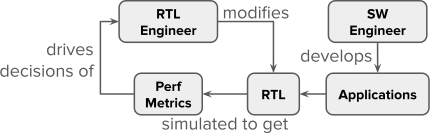
\includegraphics[width=\linewidth]{dynamic/tidalsim/uarch_iteration_flow.pdf}
  \caption{The elements of a generic eDSL.}
  \label{fig:functional_apis}
\end{figure}

% Want to consider 1) evaluation of a new microarchitectural structure, 2) optimizing the uArch of a given structure, 3) tuning hardware parameters.


% Don't want to design perf model and then design RTL to match that - what a waste, not agile!
% Also how much fidelity is typical from perf sims? (cite paper on arch simulators considered harmful). miscorrelation vs RTL *compounds* over simulation time!

\subsection{Our Contributions}

\section{Background}

% Talk about simulation methodologies
The spectrum of simulators that already exist and their limitations.

% Insert table of existing methodologies
% Cite existing perf simulators: gem5, Sniper, ZSim, SST

Why multi-level simulation?
Why not just go into perf simulators? - the correlation problem gets compounded 2x - sampling error + perf sim - RTL sim correlation errors
Aren't "trends" enough? Not when we care about small IPC changes! The absolute number matters! Also what are the special things we can get from RTL simulation that perf sim can't get us?

\section{Introduction to Multi-Level Simulation}

% Introduce the problem and your idea using *examples* and only then present the general case

\section{Implementation}

\section{Results}

\section{Related Work}

\section{Conclusion}

\begin{acks}
Acks go here (Seah, Joonho, Sophia, Chris)
\end{acks}

\bibliographystyle{ACM-Reference-Format}
\bibliography{references}

% \appendix

\end{document}
\endinput
